\documentclass[11pt]{article}

% Packages
\usepackage[utf8]{inputenc}
\usepackage{amsmath, amssymb}
\usepackage{float}
\usepackage{graphicx}
\usepackage{hyperref}
\usepackage{geometry}
\usepackage{multicol}
\usepackage{natbib} 

\geometry{margin=1in}

% Title
\title{Probabilistic Collision Cone Control Barrier Function}
\author{Maciej Różewicz}
\date{\today}

\begin{document}

\maketitle

\begin{abstract}
Safety is a fundamental requirement for autonomous systems operating in dynamic
and uncertain environments. Control Barrier Functions (CBFs) have emerged as
a~powerful tool for enforcing safety constraints in real time, but most existing
approaches assume perfect state information, which is rarely available in
practice due to sensor noise and perception errors. This paper introduces the
Probabilistic Collision Cone Control Barrier Function (PCC-CBF), a~novel
framework that explicitly accounts for uncertainty in the relative position and
velocity of obstacles by modeling them as Gaussian random variables. The
proposed method reformulates the classical collision cone condition as a~chance
constraint, ensuring that the probability of collision remains below a~specified
risk threshold. We derive tractable conditions for chance-constrained safety and
demonstrate the effectiveness of the PCC-CBF approach through simulations on
unicycle and bicycle models, as well as preliminary real-world experiments.

% The
% results show that the proposed framework enables safe and efficient navigation
% in the presence of uncertainty, providing a practical solution for robust
% autonomous operation.
\end{abstract}

\begin{multicols}{2}
%%%%%%%%%%%%%%%%%%%%%%%%%%%%%%%%%%%%%%%%%%%%%%%%%%%%%%%%%%%%%%%%%%%%%%%%%%%%%%%
\section{Introduction}
Ensuring safety is a~fundamental requirement in the design of autonomous systems, 
particularly in the context of mobile robots and self-driving vehicles operating 
in uncertain and dynamic environments.
When interacting with other traffic participants or moving obstacles, collision
avoidance must be guaranteed without compromising the ability to reach a~desired
goal. 

Among various approaches to safety-critical control, \emph{Control Barrier
Functions} (CBFs) have emerged as a~powerful tool for enforcing forward
invariance of safe sets in control-affine systems~\cite{ames2017control}. 
CBFs provide a~formal mechanism for encoding safety constraints that can be enforced 
through online quadratic programming while maintaining system performance. 
However, the majority of existing CBF-based methods assume deterministic knowledge 
of the state and environment, which is rarely available in practice due to 
sensor noise and imperfect perception.

For collision avoidance, the notion of the \emph{Collision Cone} (CC) has been 
widely used to characterize dangerous relative motions between agents~\cite{thontepu2022collision}.
The CC provides a geometric condition to determine  whether two objects are on
a~collision course, and several recent works have combined this concept with
CBFs to ensure collision-free navigation~\cite{wang2022observer}.
Yet, these approaches still rely on deterministic estimates of relative position
and velocity, making them sensitive to uncertainty. 
As perception in real-world scenarios is inherently noisy, 
such methods may yield overly conservative or unsafe behavior.

To address this limitation, in this work we propose a~\emph{Probabilistic
Collision Cone Control Barrier Function (PCC-CBF)}. 
The key idea is to extend the deterministic CC-CBF formulation by 
explicitly modeling uncertainty in relative position and velocity 
as Gaussian random variables.
This allows the safety condition to be reformulated as a~chance constraint,
ensuring that the probability of collision remains below a~specified risk threshold. 
The resulting probabilistic safety certificates can be integrated 
into a~quadratic programming framework for real-time safe control.

The main contributions of this paper are threefold:
\begin{itemize}
    \item We introduce a probabilistic formulation of Collision Cone Control
    Barrier Functions that accounts for uncertainty in perception.
    \item We derive tractable conditions for chance-constrained safety by
    exploiting Gaussian approximations of state uncertainty.
    \item We demonstrate the effectiveness of the proposed PCC-CBF approach in
    simulation studies on unicycle and bicycle models, as well as preliminary
    real-world experiments.
\end{itemize}

The remainder of this paper is organized as follows: 
Section~\ref{sec:literature} reviews related work. 
Section~\ref{sec:cbf} introduces the classical CBF framework 
and its integration with collision cones. 
Section~\ref{sec:probabilistic} presents the proposed probabilistic extension. 
Simulation and experimental results are shown in Section~\ref{sec:experiments}, 
followed by conclusions in Section~\ref{sec:summary}.

%%%%%%%%%%%%%%%%%%%%%%%%%%%%%%%%%%%%%%%%%%%%%%%%%%%%%%%%%%%%%%%%%%%%%%%%%%%%%%%
\section{Literature Review}\label{sec:literature}
The literature on safety-critical control and collision avoidance in autonomous
systems is extensive and rapidly evolving. This section reviews key developments
relevant to Control Barrier Functions (CBFs), collision cone methods, and
probabilistic safety guarantees.

\textbf{Control Barrier Functions (CBFs):}
CBFs have become a~foundational tool for enforcing safety constraints in
real-time control of nonlinear systems. The seminal work by
\citet{ames2017control} ("Control Barrier Function Methods for Safety Critical
Systems") formalized the use of CBFs for forward invariance of safe sets,
enabling
their integration into quadratic programming frameworks for safety-critical
control.
Extensions have addressed adaptive systems, input constraints, and multi-agent
scenarios~\cite{ames2019control} ("Control Barrier Functions: Theory and
Applications")
and~\cite{nguyen2016exponential} ("Exponential Control Barrier Functions for Enforcing High Relative-Degree Safety-Critical Constraints").

\textbf{Collision Cone Methods:}
The collision cone (CC) concept, originally introduced for spacecraft and
robotics applications, provides a geometric framework for predicting potential
collisions based on relative positions and
velocities~\cite{chakravarthy1998collision}
("Collision cones for motion planning and collision avoidance"). Recent works
have combined CCs with CBFs to create less conservative and more dynamically
aware safety constraints~\cite{wang2022observer} ("Observer-Based Collision Cone Control Barrier Functions for Multi-Agent Systems") and~\cite{tayal2024collisionconeapproachcontrol} ("Collision Cone Approach Control Barrier Functions for Multi-Agent Collision Avoidance"). These approaches have demonstrated improved performance in dynamic and multi-agent environments.

\textbf{Probabilistic Safety and Uncertainty:}
Most classical CBF and CC-based methods assume perfect state information,
which is unrealistic in practice. To address this, several studies have explored
robust and probabilistic extensions. Chance-constrained CBFs~\cite{black2022probabilistic} ("Probabilistic Safety for Control Barrier Functions with Applications to Adaptive Cruise Control") and~\cite{singletary2023chance} ("Chance-Constrained Control Barrier Functions for Safety-Critical Control under Uncertainty"), as well as stochastic safety certificates~\cite{dean2020guaranteeing} ("Guaranteeing Safety of Learning-Based Control Policies in Unknown Environments"), have been proposed to account for sensor noise and estimation errors. Gaussian approximations and linearization techniques are commonly used to derive tractable safety conditions under uncertainty.

\textbf{Applications:}
CBF and CC-based safety frameworks have been applied to a wide range of robotic systems, including mobile robots, autonomous vehicles, and aerial drones~\cite{ames2019control} ("Control Barrier Functions: Theory and Applications") and~\cite{wang2022observer} ("Observer-Based Collision Cone Control Barrier Functions for Multi-Agent Systems"). The integration of probabilistic safety guarantees is particularly important for real-world deployment, where perception uncertainty and dynamic obstacles are prevalent.

In summary, while CBFs and collision cone methods provide powerful tools for safety-critical control, explicitly accounting for uncertainty remains an active area of research. The proposed Probabilistic Collision Cone Control Barrier Function (PCC-CBF) builds on these foundations to offer a tractable and robust approach for safe navigation in uncertain environments.


%%%%%%%%%%%%%%%%%%%%%%%%%%%%%%%%%%%%%%%%%%%%%%%%%%%%%%%%%%%%%%%%%%%%%%%%%%%%%%%
\section{Control Barrier Function}\label{sec:cbf}
Control Barrier Functions (CBFs) are mathematical constructs used in control
theory to ensure the safety of dynamical systems. They provide a~systematic way
to enforce safety constraints by defining a~safe set of states that the system
should remain within. CBFs are particularly useful in scenarios where safety is
critical, such as in autonomous vehicles, robotics, and aerospace applications.
A~Control Barrier Function $h(x)$ is a~scalar function that maps the state space
to the real numbers. The safe set is defined as the set of states where $h(x)
\geq 0$. The boundary of the safe set is given by $h(x) = 0$, and states where
$h(x) < 0$ are considered unsafe. To ensure that the system remains within the
safe set, the CBF must satisfy certain conditions. Specifically, for a~dynamical
system described by equation (\ref{eq:control_affine_system}):
\begin{equation}
    \label{eq:control_affine_system}
    \dot{x} = f(x) + g(x)u.
\end{equation}
Where $x$ is the state, $u$ is the control input, and $f(x)$ and $g(x)$ are
system dynamics, the CBF must satisfy the following inequality (\ref{eq:safety_equation}):
\begin{equation}
    \label{eq:safety_equation}
    \dot{h}(x,u) + \alpha(h(x)) \geq 0
\end{equation}

Specifying the barrier function $h(x)$ is a~critical design choice, as it 
determines the shape of the safe set. In many robotic applications, simple 
distance-based formulations (e.g., maintaining $||p_{r}|| \geq r$ where $r$ 
is the minimum separation distance) are used to enforce collision avoidance. 
While intuitive, such constraints are often overly conservative: they do not 
account for the relative motion between agents, and may unnecessarily restrict 
the system's ability to navigate safely in dense or dynamic environments.

To address this limitation, the concept of the \emph{Collision Cone} (CC) has 
been introduced as a~geometric tool to characterize dangerous relative velocities. 
The CC describes the set of relative velocity vectors that would eventually 
lead to a collision, given the current relative position between two agents. 
Incorporating the CC into the barrier function allows one to explicitly capture 
the interplay between position and velocity, resulting in less conservative 
and more dynamically appropriate safety constraints. 

This motivates the definition of a~Collision Cone Control Barrier Function 
(CC-CBF), which encodes the requirement that the relative motion of the ego 
vehicle and obstacle remains outside the collision cone. The corresponding 
formulation is presented below.

Collision cone:
\begin{equation}
    \label{eq:collision_cone_cbf}
    h(x) = <p_{r},v_{r}> + ||p_{r}||\cdot||v_{r}||\cos{\phi}
\end{equation}
where $\cos{\phi} = \frac{\sqrt{||p_{r}||^2 - r^{2}}}{||p_{r}||}$

\cite{tayal2024collisionconeapproachcontrol}

%//////////////
The collision cone is a geometric concept used to predict potential collisions between two moving objects, such as vehicles or robots. It defines the set of relative velocity vectors that, if maintained, will eventually result in a collision given the current positions of the objects.

In more detail:

Imagine two agents: an ego vehicle and an obstacle. The relative position between them is $p_r$, and the relative velocity is $v_r$.
The collision cone is constructed by drawing lines from the ego vehicle to the edges of the obstacle, forming a cone-shaped region in velocity space.
If the relative velocity $v_r$ lies inside this cone, the ego vehicle is on a collision course with the obstacle.
If $v_r$ is outside the cone, the agents will not collide, assuming their velocities remain constant.
By incorporating the collision cone into a control barrier function, the system can enforce safety constraints that are sensitive to both position and velocity, allowing for less conservative and more flexible collision avoidance compared to simple distance-based rules. This approach is especially useful in dynamic environments where both agents may be moving.
%//////////////

Derivative of such defeined barrier function has following form:
\begin{equation}
    \label{eq:collision_cone_cbf}
    \begin{array}{c}
    \dot{h}(x,u) = <\dot{p}_{r},v_{r}> + <p_{r},\dot{v}_{r}>\\
        + <v_{r},\dot{v}_{r}> \frac{\sqrt{||p_{r}||^{2} - r^{2}}}{||v_{r}||}\\
        + <p_{r},\dot{p}_{r}> \frac{||p_{r}||}{\sqrt{||p_{r}||^{2} - r^{2}}}
    \end{array}
\end{equation}

This formula will be formulated in next section to has form as in equaltion 
\ref{eq:safety_equation}.

\begin{figure}[H]
\begin{center}
    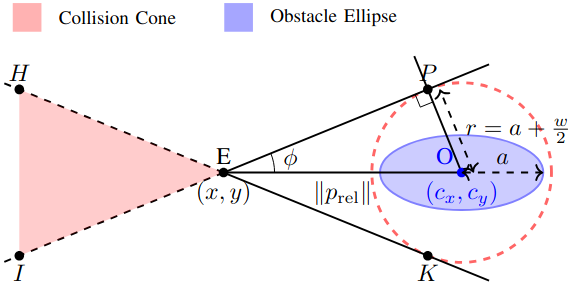
\includegraphics[width=1.0\linewidth]{fig/colision_cone_fig.png}
    \caption{Construction of collision cone for an alliptical obstacle
    considering the ego vehicle's dimensions (width $w$).} 
    \label{fig:collision_cone}
\end{center}
\end{figure}

%%%%%%%%%%%%%%%%%%%%%%%%%%%%%%%%%%%%%%%%%%%%%%%%%%%%%%%%%%%%%%%%%%%%%%%%%%%%%%%
\section{Probabilistic Collision Cone CBF}\label{sec:probabilistic}
The Collision Cone Control Barrier Function (CC-CBF) introduced in the previous
section provides a deterministic safety certificate. In particular, the condition
\eqref{eq:safety_equation} ensures that the relative motion between the robot and
an obstacle remains outside the collision cone. However, this formulation implicitly
assumes perfect knowledge of the obstacle’s position and velocity. In real-world
scenarios, perception is subject to sensor noise, occlusions, and state estimation
errors, which may lead to unsafe behavior if not explicitly accounted for.

To incorporate uncertainty, we model the relative position $p_{r}$ and velocity
$v_{r}$ of the obstacle as random variables. Let
\begin{equation}
    p_{r} = \hat{p}_{r} + \delta_{p}, \qquad
    v_{r} = \hat{v}_{r} + \delta_{v},
\end{equation}
where $\hat{p}_{r}, \hat{v}_{r}$ denote the estimated values, and $\delta_{p},
\delta_{v}$ are zero-mean Gaussian random variables with covariances
$\Sigma_{p}$ and $\Sigma_{v}$, respectively:
\begin{equation}
    \delta_{p} \sim \mathcal{N}(0, \Sigma_{p}), \qquad
    \delta_{v} \sim \mathcal{N}(0, \Sigma_{v}).
\end{equation}

By linearizing the deterministic barrier function around the estimated state
$\hat{x}$, we obtain a~first-order approximation:
\begin{equation}
    \label{eq:probabilistic_approximation}
    h(x) \approx h(\hat{x}) + \nabla_{p} h(\hat{x})^{T}\delta_{p}
    + \nabla_{v} h(\hat{x})^{T}\delta_{v}
\end{equation}
where:
\begin{itemize}
    \item $\delta_{p} \sim \mathcal{N}(0,\Sigma_{p})$ and $\delta_{v} \sim \mathcal{N}(0,\Sigma_{v})$,
    \item $\nabla_{p}h(\hat{x})^{T} = v_{r}^{T} + \frac{||v_{r}||}{\Delta}p_{r}^{T}$,
    \item $\nabla_{v}h(\hat{x})^{T} = p_{r}^{T} + \frac{\Delta}{||v_{r}||}v_{r}^{T}$,
    \item $\Delta = \sqrt{||p_{r}||^{2} - r^{2}}$.
\end{itemize}

Similarly, the derivative $\dot{h}(x,u)$ can be expressed as:
\[
    \begin{array}{c}
        \dot{h}(x,u) \approx \dot{h}(\hat{x},u) \\
         + \nabla_{p} \dot{h}(\hat{x},u)^{T}\delta_{p} + \nabla_{v} \dot{h}(\hat{x},u)^{T}\delta_{v} + \nabla_{a} \dot{h}(\hat{x},u)^{T}\delta_{a},
    \end{array}
\]
where:
\begin{itemize}
    \item $\nabla_{p} \dot{h}(\hat{x},u)^{T} = a_{r}^{T} +
    \frac{<v_{r},a_{r}>}{||v_{r}||}\frac{p_{r}}{\Delta} +
    \frac{||v_{r}||}{\Delta}v^{T} -
    \frac{||v_{r}||}{\Delta^{3}}<p_{r},v_{r}>p_{r}$,
    \item $\nabla_{v} \dot{h}(\hat{x},u)^{T} = 2v_{r} +
    \Delta\left(\frac{a_{r}}{||v_{r}||} -
    \frac{<v_{r},a_{r}>}{||v_{r}||^{3}}v_{r} \right) + \frac{1}{\Delta} \left(
    ||v_{r}||p_{r} + \frac{<p_{r}, v_{r}>}{||v_{r}||}v_{r} \right)$,
    \item $\nabla_{a} \dot{h}(\hat{x},u)^{T} = p_{r} + \frac{\Delta}{||v_{r}||}v_{r}$.
\end{itemize}

This allows us to represent the safety constraint \eqref{eq:safety_equation}
as a~random variable $c_{h}(x,u)$:
\begin{equation}
    \label{eq:safety_equation_probabilistic}
    \overbrace{
    \underbrace{\dot{h}(\dot{x},u) + \alpha(h(\dot{x},u))}_{\mu_{c_h}} + \delta_{c_{h}}
    }^{c_{h}(x,u)} \geq 0,
\end{equation}
where:
\begin{itemize}
    \item $\mu_{c_{h}}$ is the mean of $c_{h}(x,u)$ random variable,
    \item $\delta_{c_{h}}$ is a~zero-mean Gaussian random variable with variance
    $\sigma^{2}_{c_{h}} = \left( \nabla_{p} \dot{h}(\hat{x},u) + \nabla_{p} h(\hat{x}) \right)^{T} \delta_{p}
    + \left( \nabla_{v} \dot{h}(\hat{x},u) + \nabla_{v} h(\hat{x}) \right)^{T} \delta_{v} + \nabla_{a} \dot{h}(\hat{x},u)^{T}\delta_{a}$.
\end{itemize}

%  and variance $\sigma^{2}_{c_{h}} = \left( \nabla_{p} \dot{h}(\hat{x},u) + \nabla_{p} h(\hat{x}) \right)^{T} \delta_{p}
%     + \left( \nabla_{v} \dot{h}(\hat{x},u) + \nabla_{v} h(\hat{x}) \right)^{T} \delta_{v} + \nabla_{a} \dot{h}(\hat{x},u)^{T}\delta_{a}$.

Instead of requiring $c_{h}(x,u) \geq 0$ deterministically, we impose a~chance
constraint:
\begin{equation}
    \mathbb{P}\left[ c_{h}(x,u) \geq 0 \right] \geq 1 - \nu,
    \label{eq:chance_constraint}
\end{equation}
where $\nu \in (0,1)$ denotes the acceptable risk level.
Under the Gaussian approximation, condition \eqref{eq:chance_constraint} is equivalent to
\begin{equation}
    \mu_{c_{h}} - \Phi^{-1}(1-\nu) \sigma_{c_{h}} \geq 0,
    \label{eq:final_condition}
\end{equation}
where $\Phi^{-1}$ is the inverse standard normal cumulative distribution function.
This yields a~tractable inequality constraint that can be incorporated into the
quadratic program used for CBF-based control.

Equation \eqref{eq:final_condition} constitutes the proposed
\emph{Probabilistic Collision Cone Control Barrier Function (PCC-CBF)}.
It ensures that the system maintains safety with probability at least $1-\nu$,
while explicitly accounting for uncertainty in perception.

%%%%%%%%%%%%%%%%%%%%%%%%%%%%%%%%%%%%%%%%%%%%%%%%%%%%%%%%%%%%%%%%%%%%%%%%%%%%%%%
\section{Experiments}\label{sec:experiments}
Experiments were planned in two steps: first simulations - implemented in MATLAB
Autonomous Driving Toolbox, second on real robots.

    %==========================================================================
    \subsection{Motion Models}
    Two types of robot models are commonly encountered in industrial practice.
    The first is the unicycle model, typically used for indoor mobile robots.
    The second is the bicycle model, which serves as a~standard representation
    for cars in driver assistance systems and autonomous driving applications.
    
        %----------------------------------------------------------------------
        \subsubsection{Unicycle Model}
        The unicycle kinematic model is a~simple yet effective representation
        for differential-drive robots and other mobile platforms that can move
        forward and rotate, but cannot move sideways. The model captures the
        essential nonholonomic constraint that the robot's velocity is always
        aligned with its heading direction.

        In this model, the state vector consists of the position $(x_p, y_p)$ of
        the robot in the plane, its orientation $\theta$, linear velocity $v$,
        and angular velocity $\omega$. The control inputs are the linear
        acceleration $a$ and angular acceleration $\delta$.

        The continuous-time kinematic equations for the unicycle model are:
        \begin{equation}
            \label{eq:unicycle_model}
            \underbrace{
            \begin{bmatrix}
                \dot{x}_{u}\\
                \dot{y}_{u}\\
                \dot{\theta}_{u}\\
                \dot{v}_{u}\\
                \dot{\omega}_{u}
            \end{bmatrix}
            }_{\dot{x}_{u}}
            =
            \underbrace{
            \begin{bmatrix}
                v_{u}\cos{\theta_{u}}\\
                v_{u}\sin{\theta_{u}}\\
                \omega_{u}\\
                0\\
                0
            \end{bmatrix}
            }_{f_{u}(x_{u})}
            +
            \underbrace{
            \begin{bmatrix}
                0   &   0\\
                0   &   0\\
                0   &   0\\
                1   &   0\\
                0   &   1
            \end{bmatrix}
            }_{g_{u}(x_{u})}
            \underbrace{
            \begin{bmatrix}
                a_{u}\\
                \delta_{u}
            \end{bmatrix}
            }_{u_{u}}.
        \end{equation}

        \begin{figure}[H]
        \begin{center}
            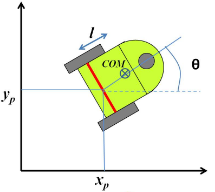
\includegraphics[width=0.7\linewidth]{fig/unicycle_model.png}
            \caption{Schematic of unicycle model.} 
            \label{fig:collision_cone}
        \end{center}
        \end{figure}


        \textbf{State:}
        The state vector is given by:
        \[
            x_{u} =
            \begin{bmatrix}
                x_{u} & y_{u} & \theta_{u} & v_{u} & \omega_{u}
            \end{bmatrix}^{T},
        \]
        where $(x_{u}, y_{u})$ represents the position, $\theta_{u}$ the heading
        angle, $v_{u}$ the linear velocity, and $\omega_{u}$ the angular velocity.

        \textbf{Control:}
        The control input vector is given by:
        \[
            u_{u} = 
            \begin{bmatrix}
                a_{u} & \delta_{u}
            \end{bmatrix}^{T},
        \]
        where $a_{u}$ is the linear acceleration and $\delta_{u}$ is the angular
        acceleration.

        This model is widely used in robotics for motion planning and control
        due to its simplicity and ability to capture the key motion constraints
        of many ground vehicles.        

        %----------------------------------------------------------------------
        \subsubsection{Bicycle Model Model}
        The bicycle model is a~widely used kinematic representation for car-like
        vehicles, capturing the essential nonholonomic constraints and steering
        dynamics. In this model, the vehicle is abstracted as a~single-track
        system with a~front steering wheel and a~rear driving wheel. The state
        vector typically includes the position $(x_p, y_p)$ of the vehicle's
        reference point (often the rear axle midpoint), the heading angle
        $\theta$, the longitudinal velocity $v$, and the yaw rate $\omega$. The
        control inputs are the longitudinal acceleration $a$ and the steering
        angle rate $\delta$.

        The continuous-time kinematic bicycle model is given by:
        \begin{equation}
            \label{eq:bicycle_model}
            \underbrace{
            \begin{bmatrix}
                \dot{x}_{b}\\
                \dot{y}_{b}\\
                \dot{\theta}_{b}\\
                \dot{v}_{b}
            \end{bmatrix}
            }_{\dot{x}_{b}}
            =
            \underbrace{
            \begin{bmatrix}
                v\cos{\theta}\\
                v\sin{\theta}\\
                0\\
                0
            \end{bmatrix}
            }_{f_{b}(x_{b})}
            +
            \underbrace{
            \begin{bmatrix}
                0   &   -v_{b}\sin{\theta_{b}}\\
                0   &   -v_{b}\cos{\theta_{b}}\\
                0   &   \frac{v_{b}}{L}\\
                1   &   0
            \end{bmatrix}
            }_{g_{b}(x_{b})}
            \underbrace{
            \begin{bmatrix}
                a_{b}\\
                \delta_{b}
            \end{bmatrix}
            }_{u_{b}}
        \end{equation}
        where $L$ is the wheelbase (distance between front and rear axles).

        \begin{figure}[H]
        \begin{center}
            
\includegraphics[width=1.0\linewidth]{fig/bicycle_model.png}
            \caption{Schematic of bicycle model.} 
            \label{fig:collision_cone}
        \end{center}
        \end{figure}

        \textbf{State:}
        The state vector is given by:
        \[
            x_{b} =
            \begin{bmatrix}
                x_{b} & y_{b} & \theta_{b} & v_{b}
            \end{bmatrix}^{T},
        \]
        where $(x_{b}, y_{b})$ represents the position, $\theta_{b}$ the heading
        angle, and $v_{b}$ the longitudinal velocity.

        \textbf{Control:}
        The control input vector is given by:
        \[
            u_{b} =
            \begin{bmatrix}
                a_{b} & \delta_{b}
            \end{bmatrix}^{T},
        \]
        where $a_{b}$ is the longitudinal acceleration and $\delta_{b}$ is the
        steering angle rate.

        This model captures the coupling between steering and heading,
        and is commonly used for path planning and control in autonomous
        driving applications.
        
    %==========================================================================
    \subsection{Simulations}
    MATLAB, Autonomous Driving
    %==========================================================================
    \subsection{Real Experiments}

%%%%%%%%%%%%%%%%%%%%%%%%%%%%%%%%%%%%%%%%%%%%%%%%%%%%%%%%%%%%%%%%%%%%%%%%%%%%%%%
\section{Summary}\label{sec:summary}

%%%%%%%%%%%%%%%%%%%%%%%%%%%%%%%%%%%%%%%%%%%%%%%%%%%%%%%%%%%%%%%%%%%%%%%%%%%%%%%
\bibliographystyle{abbrv}
\bibliography{refs}

\end{multicols}
\end{document}